\documentclass[10pt,aspectratio=169]{beamer}

\usetheme{metropolis}           % Use metropolis theme
\title{GFS Mathematik Lineare Algebra \& Computergrafik}
\date{20. Januar 2023}
\author{Valentin Zwerschke}
\institute{Königin-Olga-Stift Gymnasium}

\def\titlepage{%
  \usebeamertemplate{title page}%<---
}

\graphicspath{ {./images/} }

\usepackage{tikz}
\usepackage[german]{babel} % German

\begin{document}
  \maketitle

  \setbeamercolor{background canvas}{bg=white} % Set beamer color white bc of the white imgs

  \begin{frame}{Gliederung}
	\setbeamertemplate{section in toc}[sections numbered]
	\setbeamertemplate{subsection in toc}[subsections numbered]
	\tableofcontents[hideallsubsections]
  \end{frame}

  \section{Vektoren}
  \subsection{Vektoren}
  \begin{frame}{Vektoren}
    \begin{minipage}{10cm}
      \begin{itemize}
        \item Liste von Elementen/Zahlen $\rightarrow$ Punkte im Raum können über Vektoren beschrieben werden (Ortsvektor)
        \item Vektor Koordinaten $v_x$ und $v_y$ (Kartesisches Koordinatensystem = Achsen Senkrecht)\\\vspace{0.2cm} 
        \hspace{0.3cm}$\vec{v} = \begin{pmatrix} v_x\\ v_y\end{pmatrix}$
        \vspace{0.2cm}
        \item Länge (euklidische Norm) bsp. 2D, 3D\\
        \hspace{0.3cm}$\|\vec{v}\| =  \sqrt{v_x^2 + v_y^2}$\\
        \hspace{0.3cm}$\|\vec{v}\| =  \sqrt{v_x^2 + v_y^2 + v_z^2}$
        \vspace{0.2cm}
        \item Richtung/Normierter Vektor\\
        \hspace{0.25cm}\Large$\frac{\vec{v}}{\|\vec{v}\|}$\normalsize
        \item Richtungsvektoren sind nicht unbedingt an Ursprung gesetzt
      \end{itemize}  
    \end{minipage}
    \begin{minipage}[c]{3cm}
      \begin{tikzpicture}
        \draw[thick,->] (0,0) -- (3.5,0) node[anchor=north west] {x};
        \draw[thick,->] (0,0) -- (0,2.5) node[anchor=south east] {y};
        \draw[thick,->, blue] (0,0) -- node[above] {$\vec{v}$} (3,2) node[anchor=north east] {};
        \draw[densely dotted]  (3,0) node[below] {$v_x$} -- (3,2);
        \draw[densely dotted]  (0,2) node[left] {$v_y$} -- (3,2);
        %\node [black] at (3,2) {\textbullet};
      \end{tikzpicture}
    \end{minipage}
  \end{frame}

  \subsection{Rechnen mit Vektoren}
  \begin{frame}{Rechnen mit Vektoren}
    \vspace{0.2cm}
    \begin{minipage}{7.5cm}
      \textbf{Addition}
      \begin{itemize}
        \item Jeweils Summe der Koordinaten\\
        \vspace{0.2cm}
        \hspace{0.2cm}
        $\vec{u} + \vec{v} = \begin{pmatrix}u_x + v_x\\ u_y + v_y\end{pmatrix}$
        \vspace{-0.5cm}
      \end{itemize}
      \hspace{0.25cm}
      \begin{tikzpicture}
        \draw[thick,->] (0,0) -- (3.5,0) node[anchor=north west] {x};
        \draw[thick,->] (0,0) -- (0,2.5) node[anchor=south east] {y};

        \draw[thick,->, blue] (0,0) -- node[above] {$\vec{u}$} (3,1);
        \draw[thick,->, blue] (3,1) -- node[above] {$\vec{v}$} (1.5,2);
        \draw[thick,->, red]   (0,0) -- node[above] {\hspace{1.4cm}\small$\vec{u} + \vec{v}$} (1.5,2);
      \end{tikzpicture}
    \end{minipage}
    \begin{minipage}{6cm}
      \textbf{Subtraktion}
      \begin{itemize}
        \item Jeweils Differenz der Koordinaten\\
        \vspace{0.2cm}
        \hspace{0.2cm}
        $\vec{v} - \vec{u} = \begin{pmatrix}v_x - u_x\\ v_y - u_y\end{pmatrix}$
        \vspace{-0.5cm}
      \end{itemize}
      \hspace{0.25cm}
      \begin{tikzpicture}
        \draw[thick,->] (0,0) -- (3.5,0) node[anchor=north west] {x};
        \draw[thick,->] (0,0) -- (0,2.5) node[anchor=south east] {y};

        \draw[thick,->, blue] (0,0) -- node[above] {$\vec{u}$} (3,1);
        \draw[thick,->, red] (3,1) -- node[above] {\hspace{0.5cm}\small$\vec{v} - \vec{u}$} (1.5,2);
        \draw[thick,->, blue]   (0,0) -- node[above] {$\vec{v}$} (1.5,2);
      \end{tikzpicture}
    \end{minipage}
    \textbf{Skalierung}\\
    \hspace{1cm}
    $\lambda \vec{v} = \begin{pmatrix}\lambda v_x\\ \lambda v_y\end{pmatrix}$
    
  \end{frame}


  \subsection{Skalarprodukt}
  \begin{frame}{Skalarprodukt}
    \begin{minipage}{9cm}
      \begin{itemize}
        \item Abbildung zweier Vektoren auf einen Skalar (Zahl)
        \item Skalarprodukt:\\
        $\vec{u}\cdot\vec{v} = u_xv_x + u_yv_y$; im 2D\\
        $\vec{u}\cdot\vec{v} = u_xv_x + u_yv_y + u_zv_z$; im 3D\\
        \item Winkel zwischen $\vec{u}$ und $\vec{v}$:\\
        \hspace{0.7cm}$\vec{u} \cdot \vec{v} = \cos(\phi)\|\vec{u}\|\|\vec{v}\|$
        \item Orthogonalität genau dann wenn:
        \hspace{0.7cm}$\vec{v} \perp \vec{u} \Leftrightarrow \vec{u} \cdot \vec{v} = 0$
        \item Orthogonale Vektoren zu $\vec{v}$:\\
        \vspace{0.1cm}\hspace{0.7cm}$\lambda \small\begin{pmatrix}v_y\\ -v_x\end{pmatrix}$, \small mit $\lambda \neq 0$
      \end{itemize}
    \end{minipage}
    \begin{minipage}{4cm}
      \textbf{Interpretation}\\
      \footnotesize Produkt der Länge $\vec{v}$ mit Länge Projektion von $\vec{u}$ auf $\vec{v}$ (hier: $s$)\\
      \vspace{0.1cm}
      \begin{tikzpicture}
        \draw[thick,->] (0,0) -- (3.5,0) node[anchor=north west] {x};
        \draw[thick,->] (0,0) -- (0,2.5) node[anchor=south east] {y};
        \draw[thick,->] (0.5,0.5) -- node[above] {$\vec{u}$} (2,2);
        \draw[thick,->] (0.5, 0.5) -- node[above] {$\vec{v}$} (3,0.5);
        \draw[thick,<->, blue] (0.5, 0.35) -- node[below] {$s$} (2,0.35);
        \draw[densely dotted]  (2,0.5) -- (2,2);
        
      \end{tikzpicture}
    \end{minipage}
  \end{frame}

  \subsection{Kreuzprodukt}
  \begin{frame}{Kreuzprodukt}
    \begin{minipage}{10cm}
      \begin{itemize}
        \item Abbildung zweier Vektoren $\vec{u}$ und $\vec{v}$ im 3D Raum auf einen Vektor $\vec{w}$\\\vspace{0.25cm}
        \hspace{0.3cm}$\vec{w} = \vec{u} \times \vec{v} = \begin{pmatrix}u_x\\ u_y\\u_z\end{pmatrix} \times \begin{pmatrix}v_x\\v_y\\v_z\end{pmatrix} = \begin{pmatrix}u_yv_z - u_zv_y\\u_zv_x - u_xv_z\\u_xv_y - u_yv_x\end{pmatrix}$ 
        \vspace{0.25cm}
        \item Eigenschaften:
        \begin{itemize}
          \item $\vec{w} \perp \vec{u}$ \hspace{0.1cm}$\wedge$\hspace{0.1cm} $\vec{w} \perp \vec{v}$ (\textit{Rechte Hand Regel})
          \item $\|\vec{w}\| = \|\vec{u}\|\vec{v}\|\sin(\phi)$, mit $\phi$ Winkel zwischen $\vec{u}$ und $\vec{v}$\\
          Entspricht der Fläche, des von $\vec{u}$ und $\vec{v}$ aufgespannten Parallelogramms
        \end{itemize}
      \end{itemize}  
    \end{minipage}
    \begin{minipage}{3cm}
      \begin{tikzpicture}
        \draw[thick,->] (0,0) -- (3.5,0) node[anchor=north west] {x};
        \draw[thick,->] (0,0) -- (0,2.5) node[anchor=south east] {y};

        \draw[thick,->, blue] (0.5,1) -- node[above] {$\vec{v}$} (1.5,2);
        \draw[thick,->, blue] (0.5,1) -- node[below] {$\vec{u}$} (2.5,0.5);
        
        \draw[thick, magenta] (1.5,2) -- (3.5,1.5);
        \draw[thick, magenta] (2.5,0.5) -- (3.5,1.5);

        \node [black] at (2,1.25) {\small$||\vec{u} \times \vec{v}||$};
      \end{tikzpicture}
    \end{minipage}
  \end{frame}

  \section{Polygonale Netze}
  \subsection{Vertex, Kante, Facette, Oberfläche}
  \begin{frame}{Vertex, Kante, Facette, Oberfläche}
    \hspace{0.65cm}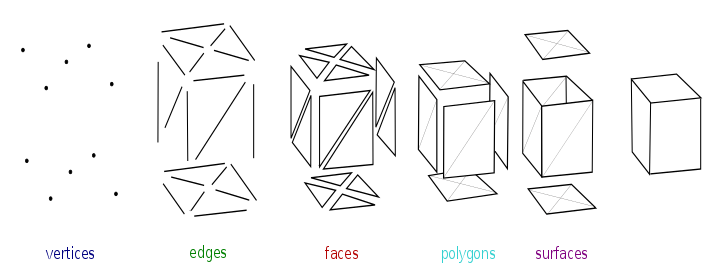
\includegraphics[scale=0.5]{mesh}
    \begin{center}
      \footnotesize \url{https://commons.wikimedia.org/wiki/File:Mesh_overview.svg}  
    \end{center}
  \end{frame}

  \subsection{Beispiel einer Oberfläche}
  \begin{frame}{Beispiel einer Oberfläche}
    \begin{center}
      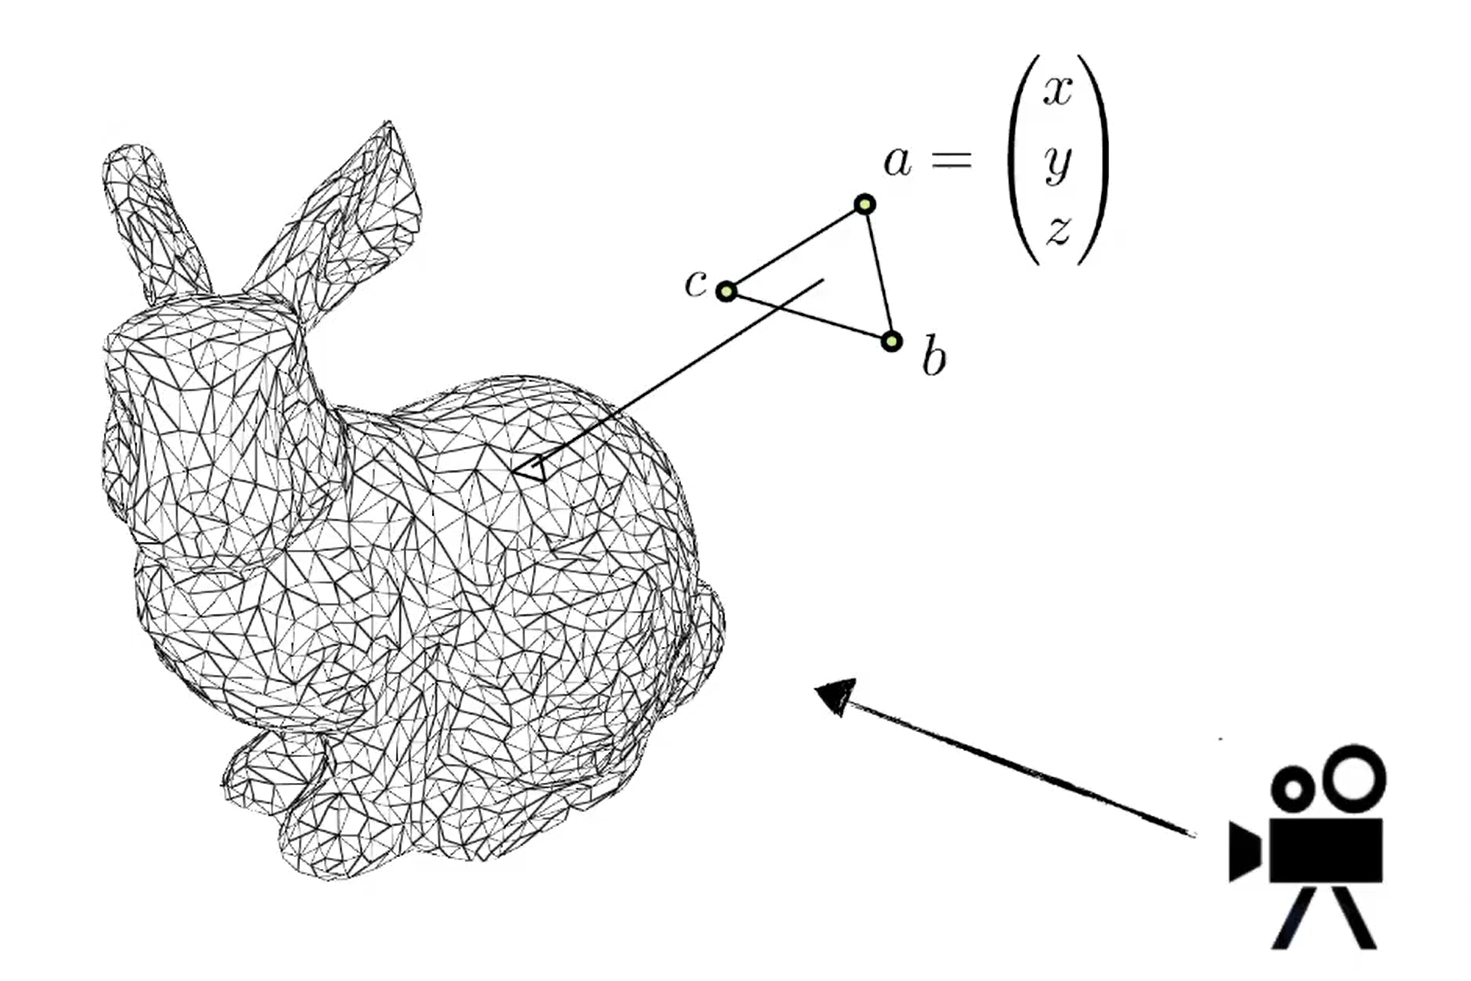
\includegraphics[scale=0.125]{bunny}
    \end{center}
    \textbf{Fragestellung der Computergrafik:}\\
    Abbildung der 3D Oberfläche auf die 2D Bildebene der Kamera\\
    (Kameraperspektive, Schattierung, ... )
  \end{frame}


  \subsection{Flächennormale}
  \begin{frame}{Flächennormale}
    \begin{minipage}{8cm}
      \normalsize
      \textbf{Der Normalenvektor zu einer Facette:}
      \begin{itemize}
        \item Senkrecht zur Facette mit Länge 1
        \item Wichtig, z.B. für Schattierungsberechnung
        \item Berechnung aus der Ortsvektoren, $\vec{a}, \vec{b}, \vec{c}$ der Vertices
        \item Kreuzprodukt der Richtungsvektoren $\vec{u}$ und $\vec{v}$
      \end{itemize}
      
      \vspace{0.2cm}
      \hspace{0.3cm}
      \large $\vec{n} = \frac{\vec{u} \times \vec{v}}{||\vec{u} \times \vec{v}||} = \frac{(\vec{b} - \vec{a}) \times (\vec{c} - \vec{a})}{||(\vec{b} - \vec{a}) \times (\vec{c} - \vec{a})||}$  
    
      
    \end{minipage}
    \begin{minipage}{3cm}
      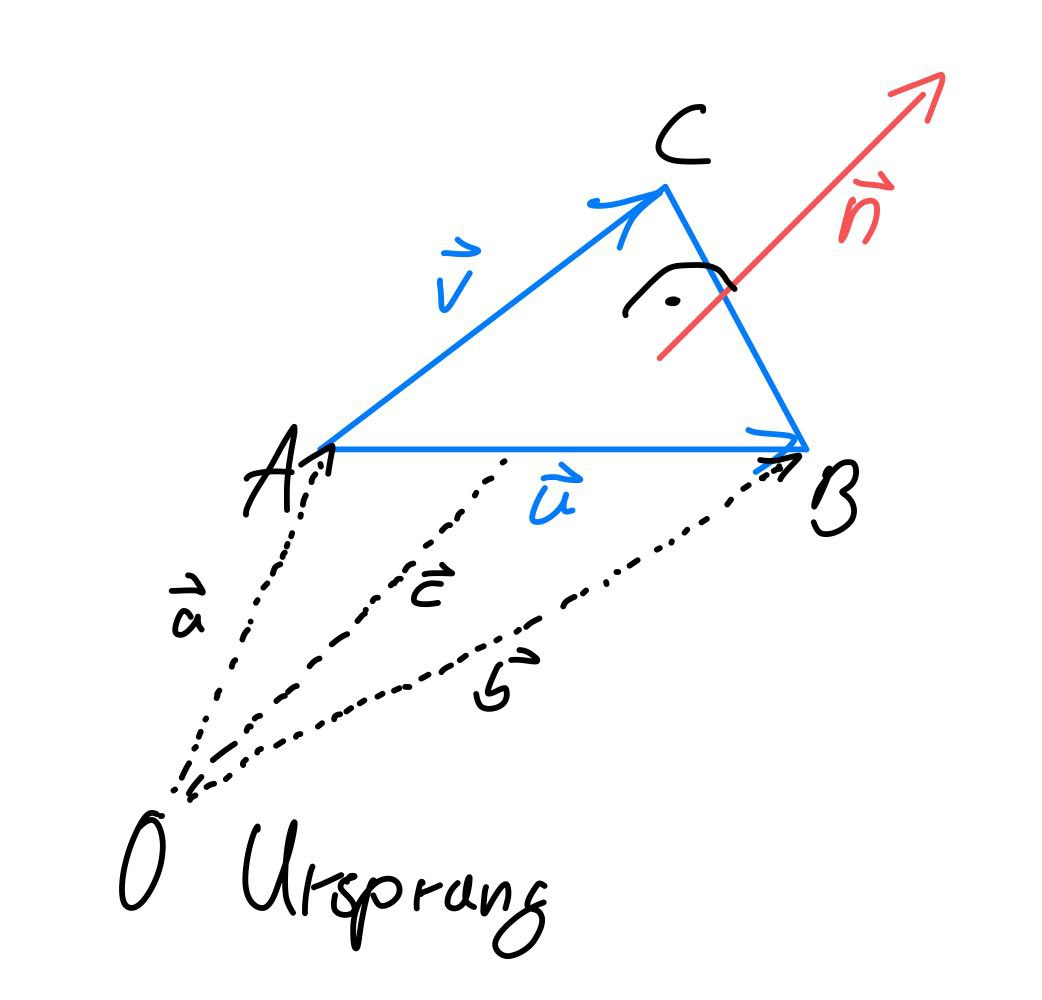
\includegraphics[scale=0.125]{sketch_n_vec}  
    \end{minipage}
  \end{frame}


  \subsection{Gerade, bzw. Strahl}
  \begin{frame}{Gerade, bzw. Strahl}
    \begin{minipage}{8cm}
      \textbf{Gerade, bzw. Strahl}
      \begin{itemize}
        \item Menge aller Punkte auf eine Linie
        \item Definiert durch zwei Punkte im Raum
        \item Darstellung in Vektorform: $g: \vec{p} + \lambda \cdot \vec{v}$
        \begin{itemize}  
          \item Aufvektor/Ortsvektor $\vec{p}$
          \item Richtungsvektor $\vec{v}$
          \item Laufvaribale $\lambda$
        \end{itemize}
        \item \textbf{Anwendungsbeispiel:}\\Unter welchem Winkel trifft ein\\Lichtstrahl auf eine Facette?
      \end{itemize}  
    \end{minipage}
    \begin{minipage}{4cm}
      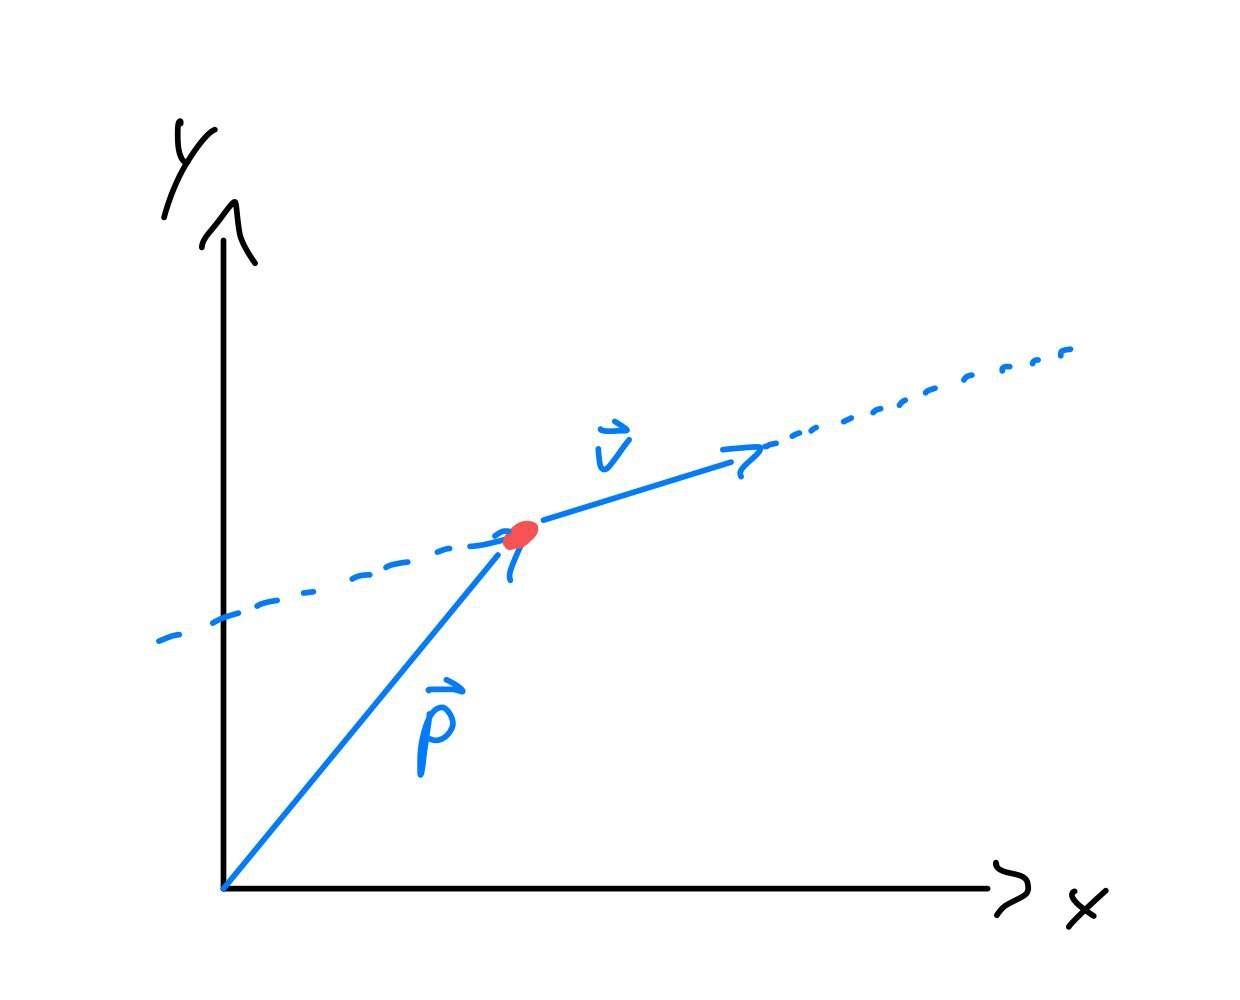
\includegraphics[scale=0.125]{sketch_gerade}
    \end{minipage}
  \end{frame}

  \subsection{Ebene}
  \begin{frame}{Ebene}
    \begin{minipage}{8cm}
      \textbf{Ebene}
      \begin{itemize}
        \item Menge aller Punkte auf einer Ebene
        \item Definiert durch drei Punkte im Raum
        \item Darstellung in Vektorform: $E: \vec{p} + \lambda_u \cdot \vec{u} + \lambda_v \cdot \vec{v}$
        \begin{itemize}  
          \item Aufvektor/Ortsvektor $\vec{p}$
          \item Richtungsvektoren $\vec{v}, \vec{u}$ (Spannvektoren)
          \item Laufvaribalen $\lambda_u$ und $\lambda_v$
        \end{itemize}
        \item \textbf{Anwendungsbeispiel:}\\Bildebene einer Kamera
        \item \textbf{Alternativ:} Normalenform der Ebene:\\
        $E: (\vec{x} - \vec{p}) \cdot \vec{n} = 0$
      \end{itemize}  
    \end{minipage}
    \begin{minipage}{4cm}
      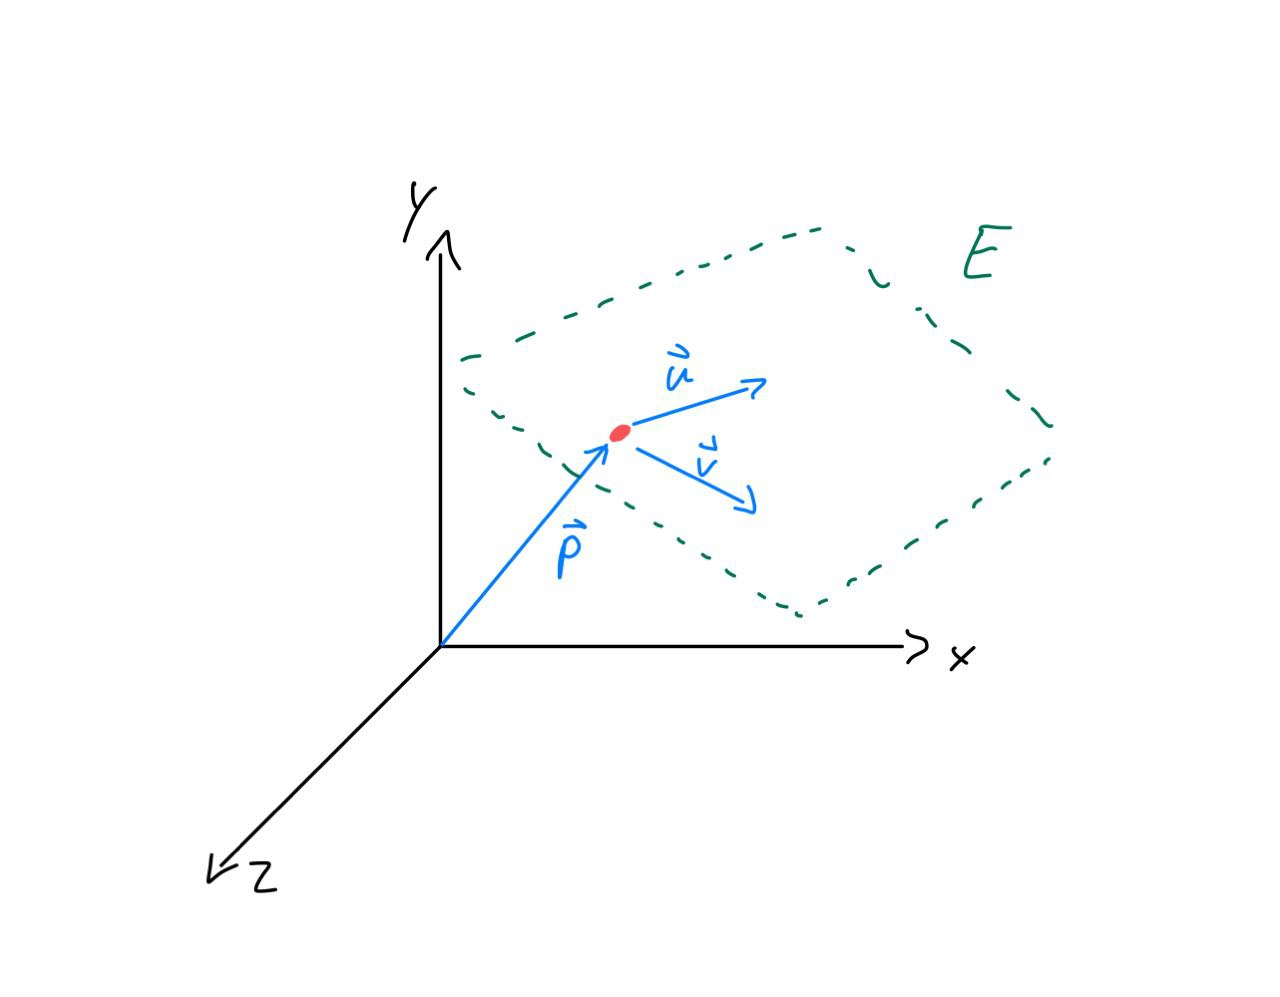
\includegraphics[scale=0.125]{sketch_ebene}
    \end{minipage}
  \end{frame}

  \section{Matrizen}

  \subsection{Matrizen}
  \begin{frame}{Matrizen}
    \begin{minipage}{9cm}
      \textbf{Matrizen}
      \begin{itemize}
        \item Rechteckige Anordung (Tabelle) von Zahlen\\ $\rightarrow$ 2D in Zeilen/Spalten
        \item Beispiel $2 \times 3$ - Matrix ("2 kreuz 3")
        \vspace{0.2cm}
        $A = \begin{pmatrix} a_{0,0} & a_{0,1} & a_{0,2}\\ a_{1,0} & a_{1,1} &  a_{1,2}\end{pmatrix}$
        \vspace{0.2cm}
        \item \textbf{Anwendungsbeispiel:} LGS\\
          $x_0 + x_1 = 18$\\
          $x_0 -2x_1 = 0$
        \item oder auch\\
        \vspace{0.2cm}
        $\begin{pmatrix}
          1 & 1\\1 & -2
        \end{pmatrix}
        \begin{pmatrix}x_0\\x_1\end{pmatrix} = \begin{pmatrix}18\\0\end{pmatrix}$
        
        \item bzw: $A \cdot \vec{x} = \vec{b}$
      \end{itemize}
    \end{minipage}
    \begin{minipage}{3cm}
      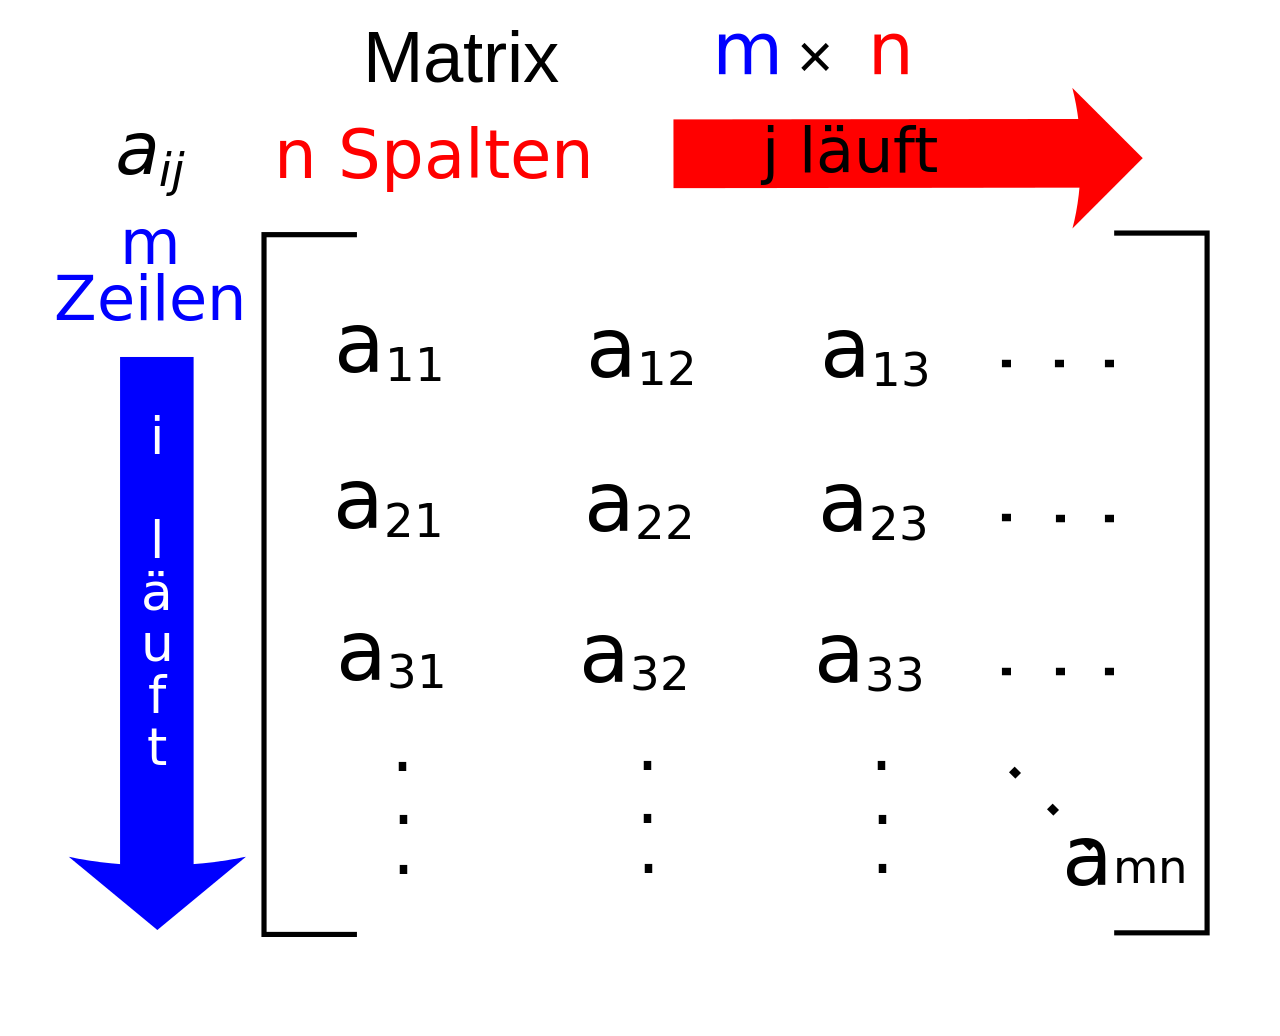
\includegraphics[scale=0.1]{matrix}
    \end{minipage}
  \end{frame}

  \subsection{Allgemeine Multiplatikation}
  \begin{frame}{Allgemeine Multiplatikation}
    \textbf{Definition Matrix Mutliplikation}
    \begin{center}
      $C = A \cdot B$ \\
      $C_{i,j} = A_{i,*} \cdot B_{*,j}$\\
    \end{center}
    \begin{itemize}
      \item Also Skalarprodukt aus Zeile $i$ der Matrix $A$ und Spalte $j$ der Matrix $B$
      \item \textbf{Achtung:} nur definiert für Matrizen, wo $A$ so viele Spalten hat wie $B$ Zeilen
    \end{itemize}
    \begin{center}
      $\begin{pmatrix}
        1 & 2 & 3\\
        4 & 5 & 6
      \end{pmatrix}
      \cdot
      \begin{pmatrix}
        1\\2\\3
      \end{pmatrix}
      = \begin{pmatrix}
        1\cdot1 + 2\cdot2 + 3\cdot3 \\
        4\cdot1 + 5\cdot2 + 6\cdot3
      \end{pmatrix} =
      \begin{pmatrix}
        14\\24
      \end{pmatrix}$\\
      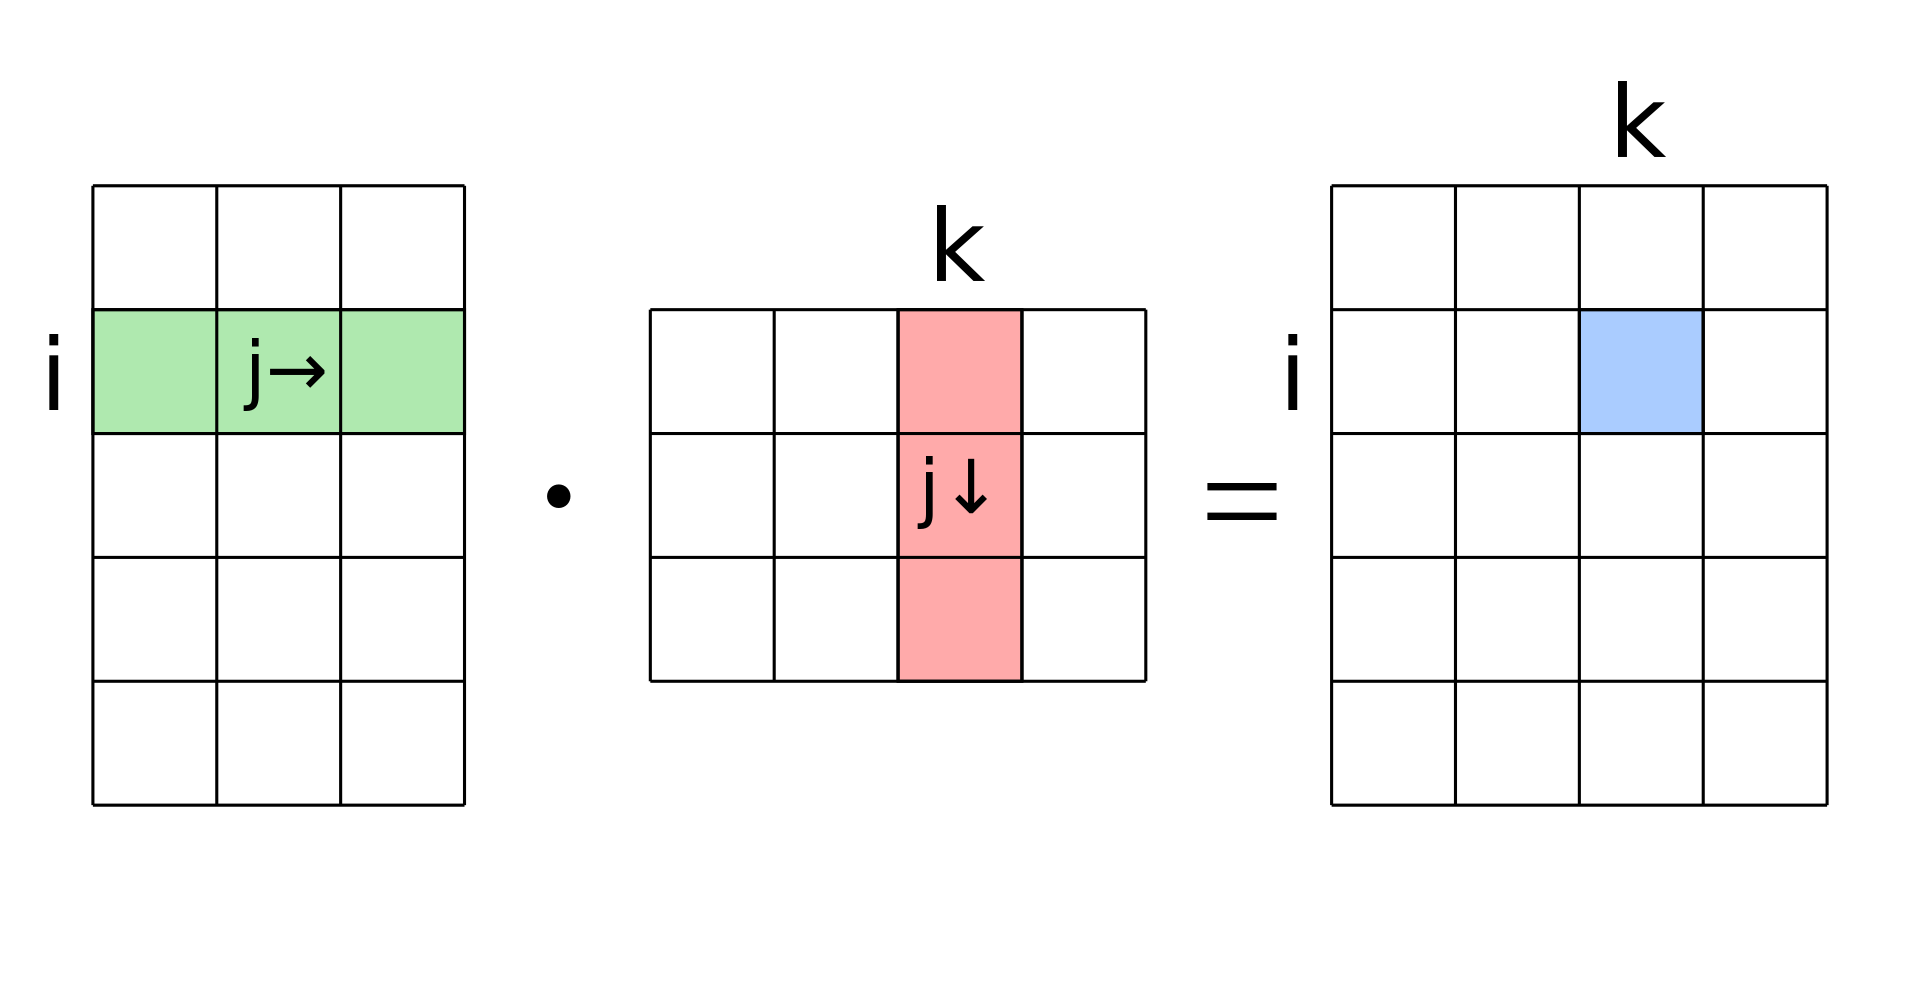
\includegraphics[scale=0.075]{matrix_mult}
    \end{center}
  \end{frame}

  \subsection{Lösung des Gleichungssystems}
  \begin{frame}{Lösung des Gleichungssystems}
    \begin{center}
      $A \cdot \vec{x} = \vec{b} \rightarrow \vec{x} = A^{-1}\vec{b}$
    \end{center}
    \begin{itemize}
      \item \textbf{Was ist Inverse Matrix?}
      \item Generell: Aufwand wächst mit 3ter Potenz der Dimension zur Berechnung der Inversen
      \item Forme für 2D:\\
      \begin{center}
        $M= \begin{pmatrix}
          a & b\\
          c & d\\
        \end{pmatrix}\hspace{0.2cm} \rightarrow \hspace{0.2cm}
        M^{-1} = \frac{1}{ad - bc}
        \begin{pmatrix}
          d & -b\\
          -c & a
        \end{pmatrix}$
      \end{center}
      \item Bsp. von vorhin:
      
        $A= \begin{pmatrix}
          1 & 1\\
          1 & -2\\
        \end{pmatrix}\hspace{0.2cm} \rightarrow \hspace{0.2cm}
        A^{-1} = -\frac{1}{3}
        \begin{pmatrix}
          -2 & -1\\
          -1 & 1
        \end{pmatrix}
        = \begin{pmatrix}
          \frac{2}{3} & \frac{1}{3}\\
          \frac{1}{3} & -\frac{1}{3}
        \end{pmatrix}
        $\\\vspace{0.25cm}
        $
        \vec{x} = 
        \begin{pmatrix}
          \frac{2}{3} & \frac{1}{3}\\
          \frac{1}{3} & -\frac{1}{3}
        \end{pmatrix}
        \cdot
        \begin{pmatrix}
          18\\
          0
        \end{pmatrix}
        =
        \begin{pmatrix}
          \frac{2}{3}\cdot18 + \frac{1}{3} \cdot 0\\
          \frac{1}{3}\cdot18 - \frac{1}{3} \cdot 0
        \end{pmatrix}
        =
        \begin{pmatrix}
          12\\
          6
        \end{pmatrix}
        $
      
    \end{itemize}
  \end{frame}

  \section{Transformation}

  \subsection{Affine Transformation: Skalierung}
  \begin{frame}{Affine Transformation: Skalierung}
    \textbf{Transformationsmatrix für Skalierung}
    \begin{center}
      $T = \begin{pmatrix}
        a & 0\\
        0 & b
      \end{pmatrix}$
      \begin{itemize}
        \item Skalierungswerte der Achens auf Hauptdiagonalen
        \item Beispiel:
        \begin{itemize}
          \item Skalierung entlang x-Achse: 1
          \item Skalerierung entlang der y-Achse: 2
            \\\vspace{0.1cm}
            $T_{1,2} = \begin{pmatrix}
              1 & 0\\
              0 & 2
            \end{pmatrix}
            $
          \begin{center}
            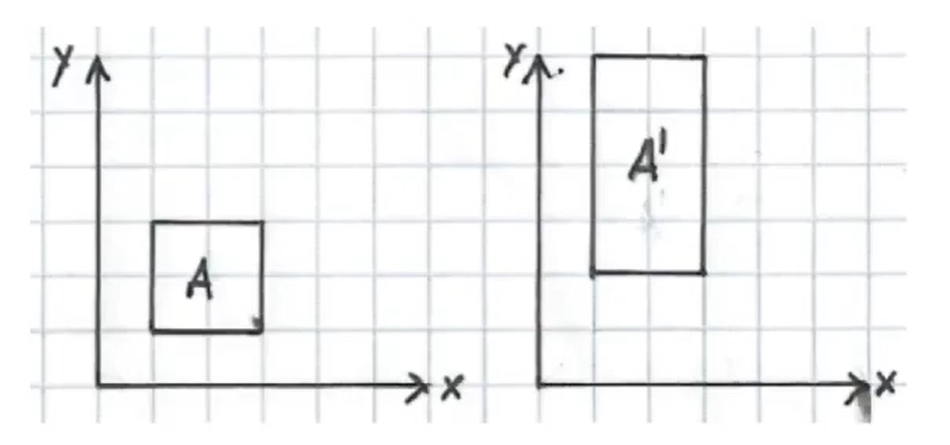
\includegraphics[scale=0.15]{skalierung}  
          \end{center}
          
          
        \end{itemize}
      \end{itemize}
    \end{center}
  \end{frame}


  \subsection{Affine Transformation: Rotation}
  \begin{frame}{Affine Transformation: Rotation}
      \begin{minipage}{9cm}
        \textbf{Transformationsmatrix für Rotation}
        \begin{center}
          $R = \begin{pmatrix}
            \cos\phi & -\sin\phi\\
            \sin\phi & \cos\phi
          \end{pmatrix}$
          \begin{itemize}
            \item Rotation um Urpsrung um den Winkel $\phi$ im 2D
            \item Beispiel:
            \begin{itemize}
              \item Vektor $\vec{v} = \begin{pmatrix}
                1\\0
              \end{pmatrix}$\\\vspace{0.1cm}
                $\vec{v}' = \begin{pmatrix}
                  \cos\phi & -\sin\phi\\
                  \sin\phi & \cos\phi
                \end{pmatrix}\begin{pmatrix}
                  1\\0
                \end{pmatrix} = \begin{pmatrix}
                  \cos\phi\\\sin\phi
                \end{pmatrix}$  
            \end{itemize}
          \end{itemize}
        \end{center}
      \end{minipage}
      \begin{minipage}{4cm}
        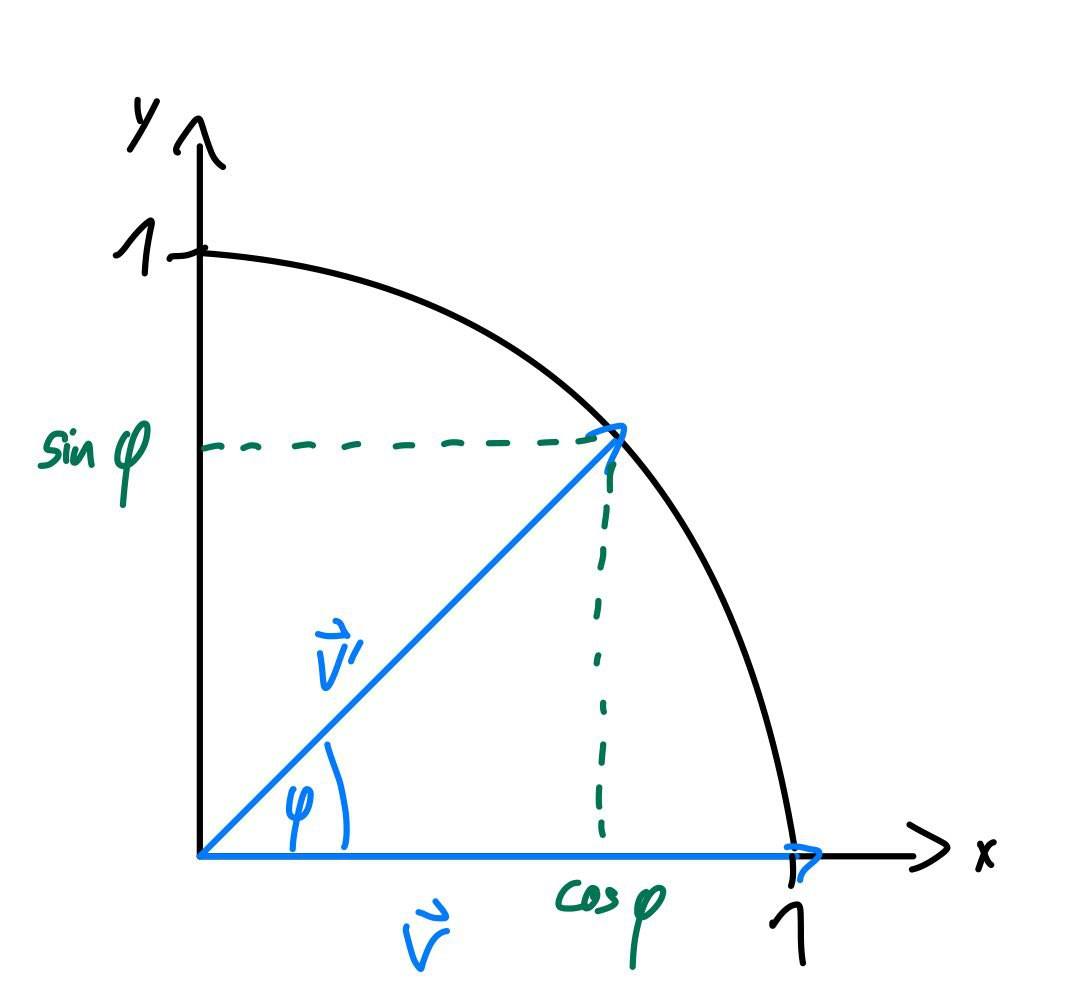
\includegraphics[scale=0.1]{rotation}  
      \end{minipage}
  \end{frame}

  \subsection{Affine Transformationen: 3D Rotation}
  \begin{frame}{Affine Transformationen: 3D Rotation}
    \begin{center}
    \begin{itemize}
      \item Um die x-Achse: \hspace{0.1cm}
      $R_x = \begin{pmatrix}
        1 & 0 & 0\\
        0 & \cos\phi & -\sin\phi\\
        0 & \sin\phi & \cos\phi
      \end{pmatrix}$\vspace{0.5cm}
      \item Um die y-Achse: \hspace{0.1cm}
      $R_y = \begin{pmatrix}
        \cos\phi & 0 & \sin\phi\\
        0 & 1 & 0\\
        -\sin\phi & 0 & \cos\phi
      \end{pmatrix}$\vspace{0.5cm}
      \item Um die z-Achse: \hspace{0.1cm}
      $R_z = \begin{pmatrix}
        \cos\phi & -\sin\phi & 0\\
        \sin\phi & \cos\phi & 0\\
        0 & 0 & 1
      \end{pmatrix}$
    \end{itemize}
  \end{center}
  \end{frame}

  \subsection{Translation/Verschiebung}
  \begin{frame}{Translation/Verschiebung}
    \textbf{Verschiebung:}
    $\vec{v}' = \vec{v} + \vec{t}$
    \begin{itemize}
      \item Anders als bei Skalierung/Rotation keine Transformationsmatrix
      \item Keine Affine Transformation (Ursprung bleibt nicht unverändert)
      \item Transformation mit Trick möglich: \textbf{Dimensionserhöhung} (w-Koordinate)
    \end{itemize}
    Vektoren: $\begin{pmatrix}
      x\\y
    \end{pmatrix}\rightarrow \begin{pmatrix}
      x\\y\\1
    \end{pmatrix}$ und $\begin{pmatrix}
      x\\y\\z
    \end{pmatrix}\rightarrow \begin{pmatrix}
      x\\y\\z\\1
    \end{pmatrix}$
    \\
    Matrizen: $\begin{pmatrix}
      a & b\\
      c & d
    \end{pmatrix}
    \rightarrow
    \begin{pmatrix}
      a & b & 0\\
      c & d & 0\\
      0 & 0 & 1
    \end{pmatrix}
    $
  \end{frame}

  \subsection{Homogene Verschiebungsmatrix}
  \begin{frame}{Homogene Verschiebungsmatrix}
    \begin{itemize}
      \item Verschiebungsvektor: $\begin{pmatrix}
        t_x\\t_y
      \end{pmatrix}$
      \item Homogene Verschiebungsmatrix: $\begin{pmatrix}
        1 & 0 & t_x\\
        0 & 1 & t_y\\
        0 & 0 & 1
      \end{pmatrix}$
      \item Test:\\\vspace{0.2cm}
      \begin{center}
        $
        \begin{pmatrix}
          x\\y
        \end{pmatrix} + 
        \begin{pmatrix}
          t_x\\t_y
        \end{pmatrix}
        =
        \begin{pmatrix}
          x + t_x\\
          y + t_y
        \end{pmatrix}
        $\\\vspace{0.2cm}$
        \begin{pmatrix}
          1 & 0 & t_x\\
          0 & 1 & t_y\\
          0 & 0 & 1
        \end{pmatrix}
        \cdot \begin{pmatrix}
          x\\y\\1
        \end{pmatrix}
        = \begin{pmatrix}
          x + t_x\\
          y + t_y\\
          1
        \end{pmatrix}
        $
      \end{center}
    \end{itemize}
  \end{frame}

  \section{Anwendung auf Computer Grafik}


  \subsection{Perspektivische Projektion}
  \begin{frame}{Perspektivische Projektion}
    \textbf{Perspektivische Projektion}
    \begin{itemize}
      \item Abbildung aus dem 3D-Raum auf die Bildebene
    \end{itemize}
    \begin{center}
      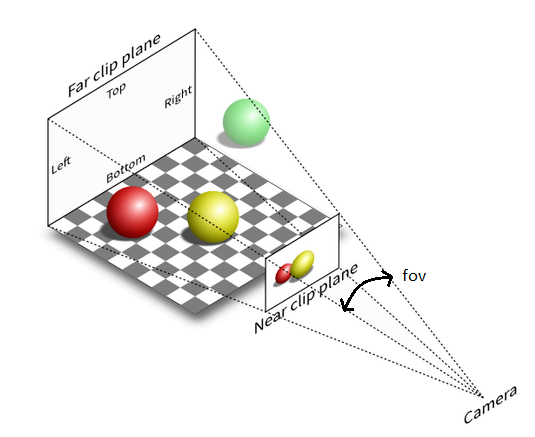
\includegraphics[scale=0.65]{projektion}  
    \end{center}
  \end{frame}


  \subsection{Perspektivische Projektion 2}
  \begin{frame}{Perspektivische Projektion 2}
    \textbf{Herleitung: Strahlensatz}\\
    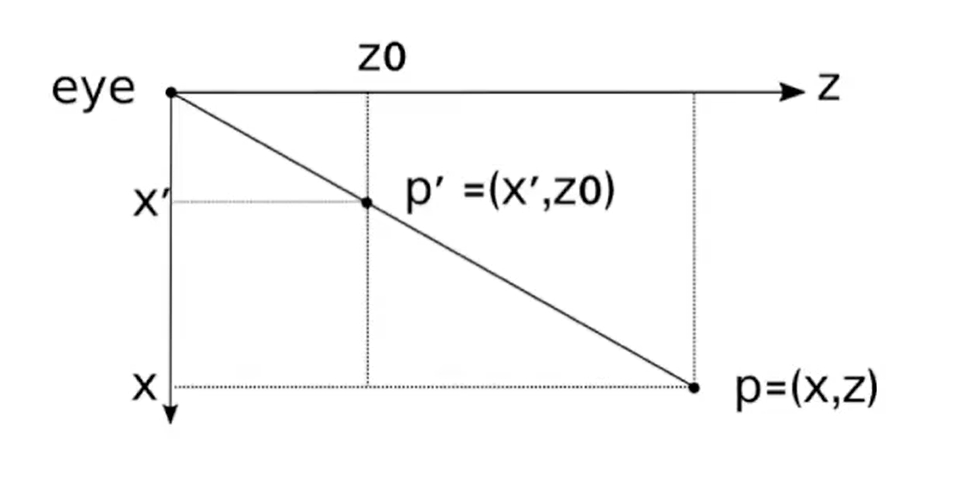
\includegraphics[scale=0.15]{strahlen}\\
    \large$\frac{z}{z_0} = \frac{x}{x'} \rightarrow x'=\frac{x\cdot z_0}{z}$\small;mit $z_0$ als Abstand zur Bildebene\\
    \normalsize
    \begin{center}
      $\begin{pmatrix}
        x'\\
        y'\\
        z_0\\
        1
      \end{pmatrix}
      =
      \begin{pmatrix}
        \frac{x\cdot z_0}{z}\\
        \frac{y\cdot z_0}{z}\\
        \frac{z\cdot z_0}{z}\\
        \frac{z}{z}\\
      \end{pmatrix}
      =
      \frac{1}{z}
      \begin{pmatrix}
        x\cdot z_0\\
        y\cdot z_0\\
        z\cdot z_0\\
        z
      \end{pmatrix}
      = \frac{1}{z}
      \begin{pmatrix}
        z_0 & 0 & 0 & 0\\
        0 & z_0 & 0 & 0\\
        0 & 0 & z_0 & 0\\
        0 & 0 & 1 & 0\\
      \end{pmatrix}
      \begin{pmatrix}
        x\\y\\z\\1
      \end{pmatrix}
      $
    \end{center}
  \end{frame}


  \subsection{Screen Mapping}
  \begin{frame}{Screen Mapping}
    \textbf{Screen Mapping Matrix mit 3 Funktionen}
    \begin{itemize}
      \item Verschiebung des Bildes auf die Mitte der Anzeigegeräts
      \item Skalierung entsprechender Brennweite $f$ der Kamera
      \item Reduzierung des 4D-homogonene Koordinaten auf 2D $\begin{pmatrix}
        x\\y
      \end{pmatrix}$\\
      $SM = \begin{pmatrix}
        f & 0 & 0 & \frac{1}{2}h\\
        0 & f & 0 & \frac{1}{2}b
      \end{pmatrix}$ mit $h$ Höhe und $b$ Breite des Ausgabegeräts
      \begin{center}        
        Bsp. Punkt $\vec{P}: \begin{pmatrix}
          1\\2\\1\\1
        \end{pmatrix}$ auf der Bildebene\\
        $SM \cdot \vec{P} = \begin{pmatrix}
          f & 0 & 0 & \frac{1}{2}h\\
          0 & f & 0 & \frac{1}{2}b
        \end{pmatrix}
        \begin{pmatrix}
          1\\2\\1\\1
        \end{pmatrix}
        = \begin{pmatrix}
          f + \frac{1}{2}h\\
          2f + \frac{1}{2}b
        \end{pmatrix}$
      \end{center}
    \end{itemize}
  \end{frame}

  \subsection{Finales Anwendungsbeispiel}
  \begin{frame}{Finales Anwendungsbeispiel}
    \textbf{Aufgabenstellung:} Ausgabe der Sicht einer Kamera auf die Facette eines Objekts
    \begin{itemize}
      \item Facette aufgspannt im 3D-Raum durch Punkte: $P_1, P_2, P_3$
      \item Ausgabe auf Monitor der Breite 4 und Höhe 3
      \item Bildebene $z_0 = 1$
      \item Kamera Sicht entlang der z-Achse mit Brennweite $f=1.5$
    \end{itemize}
    \begin{center}
      $P_1 = \begin{pmatrix}
        2\\0\\2
      \end{pmatrix}, P_2 = \begin{pmatrix}
        0\\2\\4
      \end{pmatrix},
      P_3 = \begin{pmatrix}
        1\\1\\3
      \end{pmatrix}
      $
    \end{center}
  \end{frame}

  \subsection{Finales Anwendungsbeispiel: Rechnung}
  \begin{frame}{Finales Anwendungsbeispiel: Rechnung}
    
      \textbf{Einsetzen der Punkte:}\\
      $\vec{P}_{M, 1} = SM \cdot P_{proj} \cdot \vec{P}_1$$= \begin{pmatrix}
        f & 0 & 0 & 2\\
        0 & f & 0 & 1.5
      \end{pmatrix}
      \frac{1}{z_1}
      \begin{pmatrix}
        z_0 & 0 & 0 & 0\\
        0 & z_0 & 0 & 0\\
        0 & 0 & z_0 & 0\\
        0 & 0 & 1 & 0
      \end{pmatrix}
      \begin{pmatrix}
        2\\0\\2\\1
      \end{pmatrix}
      =
      \begin{pmatrix}
        f & 0 & 0 & 2\\
        0 & f & 0 & 1.5
      \end{pmatrix}
      \begin{pmatrix}
        1\\0\\1\\1
      \end{pmatrix}
      = \begin{pmatrix}
        f + 2\\1.5
      \end{pmatrix}
      = \begin{pmatrix}
        3.5\\
        1.5
      \end{pmatrix}
      $\\
      $P_{M,2} = SM \cdot P_{proj} \cdot \vec{P}_2 = \begin{pmatrix}
        2\\2.5
      \end{pmatrix}$\\\vspace{0.2cm}
      $P_{M,3} = SM \cdot P_{proj} \cdot \vec{P}_3 = \begin{pmatrix}
        2.5\\2
      \end{pmatrix}$
  \end{frame}

  \subsection{Danke für eure Aufmerksamkeit und habt ihr Fragen?}
  \begin{frame}{Danke für eure Aufmerksamkeit und habt ihr Fragen?}
    \begin{center}
      \textbf{Vielen Dank für eure Aufmerksamkeit und habt ihr Fragen?}
    \end{center}
  \end{frame}

\end{document}